\begin{figure}[htbp]
    \centering
    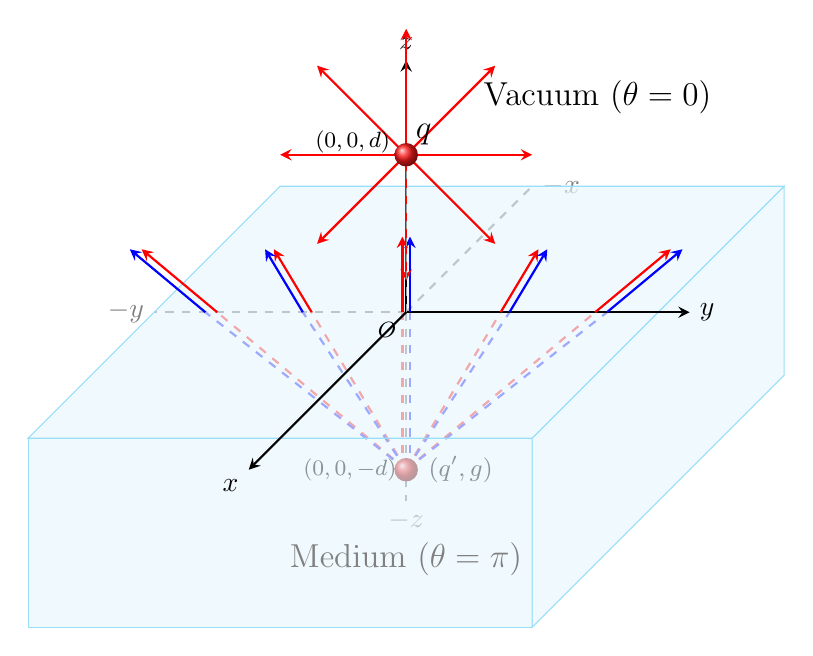
\begin{tikzpicture}[
        % 斜二测投影
        x={(-0.5cm, -0.5cm)}, 
        y={(1cm, 0cm)}, 
        z={(0cm, 1cm)}, 
        scale=0.8,
        axis/.style={->, thick, >=stealth, black},
        negaxis/.style={dashed, thick, gray},
        medium/.style={fill=cyan!10, fill opacity=0.6, draw=cyan!40, thin},
        charge/.style={shade, ball color=red!90, circle, inner sep=3pt},
        % 箭头样式:纯色,不透明
        rayRed/.style={->, >=stealth, thick, red, opacity=1},
        rayBlue/.style={->, >=stealth, thick, blue, opacity=1},
        dashRed/.style={dashed, thick, red!80},
        dashBlue/.style={dashed, thick, blue!80}
    ]
    
        % --- 参数定义 ---
        \def\limit{4}       % 平面半宽
        \def\slabH{3}       % 介质厚度
        \def\chargeH{2.5}   % 电荷高度 d
        \def\imageH{-2.5}   % 镜像电荷高度 -d
        
        % --- 1. 绘制内部/背景元素 (负坐标轴) ---
        \draw[negaxis] (0,0,0) -- (0,0,-\slabH) node[below] {$-z$};
        \draw[negaxis] (0,0,0) -- (-\limit,0,0) node[right] {$-x$};
        \draw[negaxis] (0,0,0) -- (0,-\limit,0) node[left] {$-y$};
    
        % --- 2. 绘制镜像电荷的【虚线部分】 (介质内部) ---
        % 这些线在介质内部,所以要在介质绘制之前画
        \foreach \y in {-3, -1.5, 1.5, 3} {
            % 动态偏移量计算
            \pgfmathsetmacro{\len}{sqrt(\y*\y + \chargeH*\chargeH)}
            \pgfmathsetmacro{\gap}{0.12} 
            \pgfmathsetmacro{\yshift}{(\y > 0 ? 1 : -1) * \gap * \len / \chargeH}
    
            % 红色虚线
            \draw[dashRed] (0, 0, \imageH) -- (0, \y, 0);
            % 蓝色虚线
            \draw[dashBlue] (0, 0, \imageH) -- (0, \y+\yshift, 0);
        }
        
        % --- 新增:Z轴方向的虚线 (对称微小偏移) ---
        \pgfmathsetmacro{\zGap}{0.06}
        \draw[dashRed] (0, -\zGap, \imageH) -- (0, -\zGap, 0);
        \draw[dashBlue] (0, \zGap, \imageH) -- (0, \zGap, 0);
    
        % 镜像电荷球体 (也在下方,先画)
        \node[charge] (q_img) at (0,0,\imageH) {};
        \node[anchor=west] at (0,0.2,\imageH) {\small $(q',g)$};
        % 新增坐标标注
        \node[anchor=east] at (0,0,\imageH) {\footnotesize $(0,0,-d)$};
    
    
        % --- 3. 绘制介质块 (背景) ---
        \filldraw[medium] (\limit, -\limit, 0) -- (\limit, \limit, 0) -- (\limit, \limit, -\slabH) -- (\limit, -\limit, -\slabH) -- cycle;
        \filldraw[medium] (\limit, \limit, 0) -- (-\limit, \limit, 0) -- (-\limit, \limit, -\slabH) -- (\limit, \limit, -\slabH) -- cycle;
        \filldraw[medium] (\limit, -\limit, 0) -- (\limit, \limit, 0) -- (-\limit, \limit, 0) -- (-\limit, -\limit, 0) -- cycle;
    
    
        % --- 4. 绘制正坐标轴 ---
        \draw[axis] (0,0,0) -- (\limit+1, 0, 0) node[anchor=north east] {$x$};
        \draw[axis] (0,0,0) -- (0, \limit+0.5, 0) node[anchor=west] {$y$};
        \draw[axis] (0,0,0) -- (0, 0, \limit) node[anchor=south] {$z$};
    
    
        % --- 5. 绘制镜像电荷的【实线部分】 (真空外部) ---
        % 绘制在介质之后,确保颜色鲜艳不被覆盖
        \foreach \y in {-3, -1.5, 1.5, 3} {
            % 重新计算偏移量
            \pgfmathsetmacro{\len}{sqrt(\y*\y + \chargeH*\chargeH)}
            \pgfmathsetmacro{\gap}{0.12} 
            \pgfmathsetmacro{\yshift}{(\y > 0 ? 1 : -1) * \gap * \len / \chargeH}
    
            % 红色实线
            \draw[rayRed] (0, \y, 0) -- ++(0, {0.4*\y}, {0.4*\chargeH});
            % 蓝色实线
            \draw[rayBlue] (0, \y+\yshift, 0) -- ++(0, {0.4*\y}, {0.4*\chargeH});
        }
    
        % --- 新增:Z轴方向的实线 (对称微小偏移) ---
        % 向上延伸一段距离,不完全碰到电荷 q 以免混淆
        \draw[rayRed] (0, -\zGap, 0) -- (0, -\zGap, 1.2);
        \draw[rayBlue] (0, \zGap, 0) -- (0, \zGap, 1.2);
    
    
        % --- 6. 绘制上方电荷 q 的辐射场线 ---
        \foreach \angle in {0, 45, ..., 315} {
            % 将长度从 1.2 增加到 2.5
            \draw[rayRed] (0,0,\chargeH) -- ++(0, {2*cos(\angle)}, {2*sin(\angle)});
        }
    
        % --- 7. 绘制上方电荷与标注 ---
        \draw[dashed, thin, gray!80] (0,0,0) -- (0,0,\chargeH);
        
        \node[charge] (q) at (0,0,\chargeH) {};
        \node[anchor=south west] at (q) {\large $q$};
        \node[anchor=east] at (0,-0.1,\chargeH + 0.2) {\footnotesize $(0,0,d)$};
    
        % --- 8. 区域文字标注 ---
        \node[anchor=south east] at (-2, 4, 2) {\large Vacuum ($\theta=0$)};
        \node[anchor=north west, gray] at (4, 0, -1.5) {\large Medium ($\theta=\pi$)};
        \node[anchor=north east] at (0,0,0) {\footnotesize $O$};
    
    \end{tikzpicture}
    \caption{Mirage Monopole 1}
    \label{fig:mirage_monopole_1}
\end{figure}